% !TeX encoding = UTF-8
% !TeX spellcheck = en_US
% 
\documentclass{article}

\usepackage[utf8]{inputenc}
\usepackage[T1]{fontenc} 
\usepackage[english]{babel}

\usepackage{amsmath}
\usepackage{amsthm}
\usepackage{amssymb}
\usepackage{amsfonts}
\usepackage{mathtools}
\usepackage{newtxtext}
\usepackage{newtxmath}

\usepackage{microtype}
\usepackage{floatflt}

\usepackage{graphicx}
\usepackage{caption}
\usepackage{marginnote}

\usepackage{hyperref}
\usepackage[backend=bibtex]{biblatex} %I need to use biblatex for some special features
\bibliography{bib}


\usepackage{mdframed}
\mdfsetup{skipabove=\topskip,skipbelow=\topskip}
\global\mdfdefinestyle{exampledefault}{%
	outerlinewidth=5pt,innerlinewidth=0pt,outerlinecolor=red,roundcorner=5pt
}

% ------------- Geometry ---------------------------
%\usepackage{geometry}
%\geometry{
%	a4paper,
%	total={170mm,257mm},
%	left=25mm,
%	right=25mm,
%	top=20mm,
%}
% ------------- MATHEMATICAL ENVIRONMENTS ----------
\newcommand{\R}{\mathbb{R}}
\newcommand{\C}{\mathbb{C}}
\newcommand{\tu}{\tilde{U}}
\renewcommand{\hat}{\widehat}
\renewcommand{\phi}{\varphi}
\newcommand{\E}[1]{\mathbb{E}\left[ #1 \right]}
\newcommand{\diff}{\mathop{}\!d}
\newcommand{\pd}[2]{\frac{\partial #1}{\partial #2}}
\newcommand{\pds}[2]{\frac{\partial^2 #1}{\partial #2^2}}
\renewcommand{\div}{\mathrm{div}}

\DeclarePairedDelimiter\abs{\lvert}{\rvert}%
\DeclarePairedDelimiter\norm{\lVert}{\rVert}%

\makeatletter
\let\oldabs\abs
\def\abs{\@ifstar{\oldabs}{\oldabs*}}
%
\let\oldnorm\norm
\def\norm{\@ifstar{\oldnorm}{\oldnorm*}}
\makeatother

% ------------- IMPORTARE CODICE IN MATLAB/OCTAVE --
\usepackage{listings}
\usepackage{color}
\usepackage{bigfoot} % to allow verbatim in footnote
\usepackage[numbered,framed]{matlab-prettifier}

\usepackage{filecontents}

\let\ph\mlplaceholder % shorter macro
\lstMakeShortInline"

\lstset{
	style              = Matlab-editor,
	basicstyle         = \mlttfamily,
	escapechar         = ",
	mlshowsectionrules = true,
}

\theoremstyle{definition}
\newtheorem{defn}{Definition}[section]
\theoremstyle{plain}
\newtheorem{thm}{Theorem}[section]
\newtheorem{prop}{Proposition}[section]
\newtheorem{cor}{Corollary}[section]
\newtheorem{lmm}{Lemma}[section]
\theoremstyle{remark}
\newtheorem*{recall}{Recall}
\newtheorem*{example}{Example}
\newtheorem*{remark}{Remark}


\author{Pillon, Erik}
\title{The Fokker-Planck Equation}
\date{\today}

\begin{document}
\maketitle
\begin{abstract}
	Something
	
	All the codes wer written by myself and where not explicitely said all the graphics were produced in \textsc{Matlab} or Julia v0.6.3.
\end{abstract}
We begin with a particular Fokker-Planck equation where the drift is the gradient of a given smooth potential $ V\colon\R^d\to\R $
\begin{equation}
\label{eq:fokker-planck_eq}
\begin{cases}
\pd{}{t}n(t,x)-\Delta n(t,x)-\mathrm{div}(n(t,x)\nabla V(x))=0,\qquad t\geq0,x\in\R^d,\\
n(t=0,x)=n^0(x)
\end{cases}
\end{equation}
\section{Elementary a priori estimates}
The main properties of solutions of \eqref{eq:fokker-planck_eq} are the nonnegativity principle, the ‘mass’ conservation and the existence of a non-zero steady state,
\begin{align}
	n^0\geq 0 \longrightarrow n(t,x)\geq 0,\\
	\int_{\R^d}n(t,x)\diff x=\int_{\R^d}n^0(x)\diff x, \quad \forall t\geq 0,\\
	\mu e^{-V(x)} \quad \text{are steady states for all $ \mu\in\R $.} \label{eq:steady_states}
\end{align}
this last statement is because $ \Delta e^{-V}=\div(\nabla e^{-V})=-\div(e^{-V}\nabla V) $

It is intuitive that the decay properties of this steady state should play a role, for example because its integrability is a desirable property. This relies on growth assumptions of $ V(x) $ at infinity. A potential $ V $ is called \textit{confining} if $ V(x)=\to+\infty $ as $ \abs{x}\to\infty $; typically $ V(x)=\frac{\norm{x}^2}{2} $ determines a Gaussian steady state.

A simple idea is to look directly for a priori estimates in $ L^2 $. After multiplication by $ n $ and integration by parts, one finds
\begin{align}
	\frac{1}{2}\pd{}{t}\int_{\R^d}n(t,x)^2\diff x+\int_{\R^d}\abs{\nabla n(t,x)}^2\diff x &= -\int_{\R^d}\nabla n(t,x)\nabla V(x)n(t,x)\diff x\\ù
	&=-\frac{1}{2}\int_{\R^d}\nabla n(t,x)^2\nabla V(x)\diff x
\end{align}
and thus we arrive at
\begin{equation}
\frac{1}{2}\pd{}{t}\int_{\R^d}n(t,x)^2\diff x+\int_{\R^d}\abs{\nabla n(t,x)}^2\diff x=\frac{1}{2}\int_{\R^d}n(t,x)^2\Delta V(x)\diff x.
\end{equation}
When $ \Delta V\leq -\nu<0 $, with $ \nu $ a constant, one finds that 
\[\int_{\R^d}n(t,x)^2\diff x\leq e^{-\mu}\int_{\R^d}n^0(x)^2\diff x \]
Note that, in this case, the steady state in \eqref{eq:steady_states} is not integrable and this calculation shows the interest of confining potentials.

\section{Weak Solution}
We define now a weak solution of \eqref{eq:fokker-planck_eq} by testing against a function $ \Phi\in\mathcal{D}(\R^+\times\R^d) $
\begin{equation}
\int_{0}^{\infty}\int_{\R^d}n(t,x)\left[-\pd{\Phi}{t}-\Delta\Phi+\nabla V\cdot\nabla\Phi \right]\diff x\diff t=\int_{\R^d}n^0(x)\Phi(0,x)\diff x.
\label{eq:weak_solution}
\end{equation}
We see that this makes sense under different assumptions for $ V $. Examples are
\begin{itemize}
	\item assume $ \nabla V\in L_{loc}^2(\R^d) $ and $ n\in L^{\infty}\left((0,T);L^2(\R^d)\right) $ for all $ T>0 $,
	\item assume $ \nabla V\in C(\R^d) $ and $ n\in L^{\infty}\left(\R^+;M^1(\R^d)\right) $ (bounded measure), which is relevant in view of mass conservation.
\end{itemize}
Another option is to use, as we did for the relative entropy structure, the alternative formulation
\begin{equation}
\begin{cases}
\pd{}{t}n(t,x)-\div\left(e^{-V(x)}\nabla(n(t,x)e^{V(x)})\right)=0, \qquad t\geq 0, x\in\R^d,\\
n(t=0,x)=n^0(x).
\end{cases}
\end{equation}
This leads to another possible weak formulation
\[\int_{0}^{\infty}\int_{\R^d}n(t,x)\left[-\pd{\Phi}{t}-e^{V(x)}\div\left(e^{-V(x)}\nabla\Phi \right) \right]\diff x\diff t=\int_{\R^d}n^0(x)\Phi(0,x)\diff x, \]
which is not very different from \eqref{eq:weak_solution}.

When applying the Lax-Milgram theory \cite{salsa2016equazioni} for steady states, the two formulations are however very different. The direct formulation leads to the use of the scalar product (definiteness should come from the zero order term for example)

\[((n,\Phi))_1=\int_{\R^d}\nabla n(x)\cdot \nabla\Phi(x)\diff x+\int_{\R^d}n(x)\nabla\Phi(x)\cdot\nabla V(x)\diff x. \]
The modified formulation leads to the scalar product (we use the test function $ \Phi(x)=\phi(x)e^{V(x)} $)

\[((n,\phi))_2=\int_{\R^d}\nabla(n(x)e^{V(x)})\cdot\nabla(\phi(x)e^{V(x)})e^{-V(x)}\diff x= \int_{\R^d}\nabla\tilde{n}(x)\cdot\nabla\Phi(x)e^{-V(x)}\diff x. \]
This is a self-adjoint scalar product in the Hilbert space $ H^1(e^{-V(x)}\diff x) $, with definiteness directly related to the Poincaré inequality in the full space.

\section{The Complete Fokker-Planck Equation}
The complete Fokker-Planck equation (also called the Kolmogorov equation in the theory of Markov/diffusion processes) is given by

\begin{equation}
\begin{cases}
\pd{}{t}n(t,x)-\frac{1}{2}\sum_{i,j=1}^{d}\frac{\partial^2}{\partial x_i\partial x_j}(B_{ij}(t,x)n(t,x))+\div(n(t,x)U(t,x))=0, \qquad t\geq0,x\in\R^d,\\
n(t=0,x)=n^0(x).
\end{cases}
\end{equation}
Here $ U\colon\R^+\times\R^d\to\R^d $ is the velocity field and $ B\colon\R^+\times\R^d\to\mathcal{M}_+^{d\times d} $ is the nonnegative symmetric diffusion matrix. In other words, it is always assumed to satisfy, for some constant $ \nu\geq 0 $,

\[\sum_{i,j=1}^dB_{i,j}(t,x)\xi_i\xi_j\geq\nu\abs{\xi}^2,\qquad \forall \xi\in\R^d. \]
The main properties are still the sign property
\[n^0\geq0\Rightarrow n\geq 0, \]
and 'mass' conservation
\[\int_{\R^d}n(t,x)\diff x=\int_{\R^d}n^0(x)\diff x,\qquad \forall t\geq0. \]
We assume that there is a steady state $ N(x) $ to \eqref{eq:fokker-planck_eq}

\begin{equation}
-\frac{1}{2}\sum_{i,j=1}^{d}\frac{\partial^2}{\partial x_i\partial x_j}(B_{ij}(x)N(x))+\div(N(x)U(x))=0, \qquad \forall x\in\R^d, \qquad N(x)>0.
\end{equation}
The existence of solutions depends heavily on the coefficients $ (B,U) $ and on the desired properties for $ N $ (usually $ N\in L^1\cap L^{\infty}(\R^d) $), but a typical example is as before 
\[\frac{1}{2}B=I\quad (identity matrix), \quad U(x)=-\nabla V(x), \quad N(x)=\mu e^{-V(x)},\mu\in\R. \]

More generally for a constant matrix $ B $, when $ U=-B\nabla V(x) $, we find the same steady states.

\section{Stochastic Differential Equations (SDE)}
The Fokker-Planck equation is intimately connected to Stochastic Differential Equations and we explain this in the following. We give here a very intuitive and non-rigorous construction based on numerical approximations. For a given, sufficiently smooth, vector field $ U\in\R^d $ and a matrix $ \sigma(t,x)\in M_{d,p} $, one can build the solution of the It\^{o} Stochastic Differential Equation
\begin{equation}
\begin{cases}
\diff X(t)=U(t,X(t))\diff t+\sigma(t,X(t))\diff W(t),\\
X(0)=X^0\in\R^d \qquad \text{(a random vector)}
\end{cases}
\end{equation}
with $ W(t)=\left(W^1(t),\dots,W^p(t) \right) $, $ p $ independent Brownian motions.

The numerical construction is essentially based on the numerical approximations through subsequent finite increments. This defines the Euler scheme
\begin{equation}
X^{k+1}=X^k+\Delta t U(t^k,X^k)+\sqrt{\Delta t}\sigma\left(t^k,X^k\right)Y^k.
\label{eq:num_approximation}
\end{equation}
Because the random variable $ Y^k $ is independent of $ X^k $ and $ \E{Y^k}=0 $, we have
\begin{equation}
\E{X^{k+1}-X^k}=\Delta t\E{U(t^k,X^k)},
\end{equation}
and 
\begin{align}
	\E{\left(X^{k+1}-X^k\right)^2}&= \E{\Delta t^2U^2(t^k,X^k)+2\Delta t^{3/2}U(t^k,X^k)\sigma(t^k,X^k)Y^k+\Delta t\abs{\sigma(t^k,X^k)Y^k}^2}\\
	&=\Delta t\E{\sigma^2(t^k,X^k)}\E{\left(Y_k\right)^2}+O(\Delta t^2)\\
	&=\Delta t\E{\sigma^2(t^k,X^k)}+O(\Delta t^2)
\end{align}
Except when $ \sigma\equiv0 $, this scales like the Brownian motion. The type of approximation scheme used in \eqref{eq:num_approximation} is very important, in opposition to the deterministic case. Changing this approximation also changes the limit. The Stratonovich convention is an example and the notion is denoted as
\begin{equation}
\begin{cases}
\diff X(t)=U(t,X(t))\diff t+\sigma(t,X(t))\circ\diff W(t),\\
X(0)=X^0\in\R^d \qquad \text{(a random vector)}
\end{cases}
\end{equation}
The Stratonovich SDE corresponds to the semi-implicit approximation in the stochastic term
\begin{equation}
X^{k+1}=X^k+\Delta tU(t^k,X^k)+\sqrt{\Delta t}\sigma\left(t^k,\frac{X^k+X^{k+1}}{2} \right)Y^k.
\end{equation}
It may be may approximated as
\begin{align}
	X^{k+1}&\approx X^k+\Delta tU(t^k,X^k)+\sqrt{Delta t}\left[\sigma(t^k,X^k)+\frac{1}{2}D\sigma(t^k,X^k)(X^{k+1}-X^k) \right]Y^k\\
	&\approx X^k+\Delta tU(t^k,X^k)+\frac{Delta t}{2}D\sigma(t^k,X^k)\sigma(t,X^k)(Y^k)^2+\sqrt{\Delta t}\sigma(t^k,X^k)Y^k+O(\Delta t^{3/2}).
\end{align}
This means that
\begin{equation}
\E{X^{k+1}-X^k}=\Delta t\E{U(t^k,X^k)}+\frac{\Delta t}{2}\E{D\sigma(t^k,X^k)\sigma(t^k,X^k)},
\end{equation}
In other words, one cannot take the expectation as simply as for It\^o SDE.

Because $ \E{(Y^k)^3}=0 $, we also find that
\[\E{(X^{k+1}-X^k)^2}=\Delta t\E{\sigma^2(t^k,X^k)}+O(\Delta t^2). \]
It is remarkable that the Stratonovich semi-implicit scheme leads to the same first two expectations as the It\^o formula with the drift $ U $ changed in $ U-\frac{1}{2}\sigma'\sigma $; in fact for the limit $ \Delta t\to0 $, the two constructions are equivalent with this modification for the drift. This is to say that the limit of the term $ (Y^k)^2 $ is $ 1 $ in probability.

\section{The It\^o Formula}
An important tool in the theory of SDEs is the It\^o formula that gives the equation satisfied by the random variable $ u(t,X(t)) $, when $ u\in C^2(\R^{d+1};\R) $,
\begin{equation}
\diff u(t,X(t))=\left[\frac{\partial u(t,X(t))}{\partial t} +U(t,X(t))\cdot Du(t,X(t))+\frac{1}{2}B(t,X(t))\cdot D^2u(t,X(t))\right]\diff t+\sigma(t,X(t))\cdot Du(t,X(t))\cdot\diff W(t)
\label{eq:Ito_Formula}
\end{equation}
with
\begin{equation}
B(t,x)=\frac{1}{2}\sigma(t,x)\cdot\sigma^t(t,x)\qquad \text{($\sigma^t $ denotes the transposed matrix)}.
\end{equation}
In other words, the chain rule does not apply to SDEs as it applies to ODEs $ (\sigma(t,x)=0) $ and it gives an additional term, namely the term $ B(t,X(t))\cdot D^2u(t,X(t)) $.

This formula can be derived from the approximation \eqref{eq:num_approximation}. Using Taylor’s expansion in time, we find 
\begin{align}
	u(t^{k+1},X^{k+1})&=u(t^k,X^k)+\Delta t	\pd{u(t^k,X^{k+1})}{t}+O(\Delta t^2)\\
	&=u(t^k,X^{k+1})+\Delta t\pd{u(t^k,X^k)}{t}+O(\Delta t^{3/2}).
\end{align}
Therefore, using now Taylor’s expansion in space, we find
\begin{align*}
	u(t^{k+1},X^{k+1})&=u(t^k,X^k)+\Delta t	\pd{u(t^k,X^{k})}{t}+O(\Delta t^{3/2})\\
	&+\left[\Delta tU(t^k,X^k)+\sqrt{\Delta t}\sigma(t^k,X^k)Y^k \right]\cdot Du(t^k,X^{k})\\
	&+\frac{1}{2}\Delta t\sigma^2(t^k,X^k)(Y^k)^2D^2u(t^k,X^k).
\end{align*}
As we already saw for the Stratonovich model, the limit of the term $ (Y^k)^2 $ is $ 1 $ for the limit $ \Delta t\to0 $ and we see that this is the discrete version of \eqref{eq:Ito_Formula}.
In the case of the Stratonovich convention, one can use the chain rule as in the deterministic case (and this is the advantage gained from the more complicated average)
\begin{equation}
du(t,X(t))=\left[\pd{u(t,X(t))}{t}+U(t,X(t))\cdot Du(t,X(t)) \right]\Delta t+\sigma(t,X(t))\cdot Du(t,X(t))\circ\diff W(t).
\label{eq:Stratonovich_formula}
\end{equation}
To see this, we can redo the discrete version, and to simplify, use a function of $ X $ only,
\[u(X^{k+1})=u(X^k)+Du(X^k)\left[\Delta tU(t^k,X^k)+\sqrt{\Delta t}\sigma\left(\frac{X^k+X^{k+1}}{2} \right)Y^k \right]+\frac{\Delta t}{2}D^2 u(X^k)\sigma\left(\frac{X^k+X^{k+1}}{2} \right)^2(Y^k)^2+O(\Delta t^{3/2}), \]
which we may ‘center’ to follow the semi-implicit rule
\begin{align*}
	u(X^{k+1})=u(X^k)+\Delta tDu(X^k)U(t^k,X^k)+\sqrt{\Delta t}Du\left(\frac{X^k+X^{k+1}}{2}\right)\sqrt{\Delta t}\sigma\left(\frac{X^k+X^{k+1}}{2}\right)Y^k\\
	-\frac{\sqrt{\Delta t}}{2}D^2u(X^k)(X^{k+1}-X^k)\sigma\left(\frac{X^k+X^{k+1}}{2}\right)^2Y^k\\
	+\frac{\Delta t}{2}D^2u(X^k)\sigma\left(\frac{X^k+X^{k+1}}{2}\right)^2(Y^k)^2+O(\Delta t^{3/2})
\end{align*}
and because the dominant term in $ X^{k+1}-X^k $ is $ \sqrt{\Delta t}\sigma\left(\frac{X^k+X^{k+1}}{2}\right)Y^k $, we finally end up with
\[u(X^{k+1})=u(X^k)+\Delta tDu(X^k)U(t^k,X^k)+\sqrt{\Delta t}Du\left(\frac{X^k+X^{k+1}}{2}\right)\sigma \left(\frac{X^k+X^{k+1}}{2}\right)Y^k+O(\Delta t^{3/2}), \]
which is the discrete version of \eqref{eq:Stratonovich_formula}.
\section{The Kolmogorov Equation}
To go further and make the link with the Fokker-Planck equation, we recall the
\begin{defn}
	The probability density $ n(x) $ of a random variable $ X $ is defined by the identity
	\[\int u(x)n(x)\diff x=\E{u(X(\omega))}, \]
	for all smooth test functions u with compact support.
\end{defn} 

We give the probability density $ n^0(x) $ of $ X^0 $ and we denote by $ n(t,x) $ the probability density of the process $ X(t,\omega) $. Then, we can deduce from the It\^o formula that 
\begin{thm}[Fokker-Planck-Kolmogorov Equation]
	For the process \eqref{eq:num_approximation}, the 	limiting probability density $ n(t,x) $ satisfies the Fokker-Planck equation \eqref{eq:fokker-planck_eq}.
\end{thm}



\section{Numerical Implementations}
\begin{figure}
	\centering
	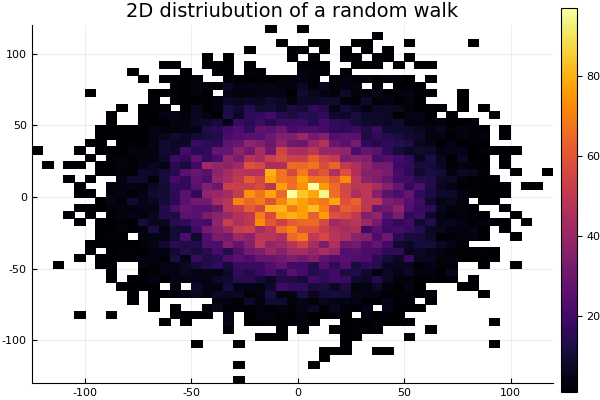
\includegraphics[width=.7\textwidth]{Code/Julia/Im/rw.png}
	\caption[2D simulation random walk]{\marginnote{\texttt{rw.jl}}Numerical simulation of a 2D random walk}
\end{figure}


% ------------ bibliography ----------------
\nocite{tuckerman2010statistical}
\nocite{perthame2015parabolic}
\nocite{salsa2016equazioni}
\printbibliography
\end{document}
